\subsection{Induktive Ladung}\label{sec:energieuebertragung}

Der Dōjō wird mit Hilfe des Induktionsprinzips geladen. Der Ladeprozess wird gestartet, sobald der Dōjō auf die Ladestation gestellt wird. Beim Induktionsprinzip wird die Energie mithilfe von Spulen über eine kurze Distanz zwischen zwei Schaltungen transportiert. Die erste Schaltung wird Transceiver genannt und sendet die Energie. Sie besteht aus einem Pulsgenerator, mit welchem das LC-Glied gepulst wird. Sie macht den Hauptanteil einer solchen induktiven Ladeschaltung aus. Die zweite Schaltung wird Receiver genannt und empfängt die Energie. Sie besteht ebenfalls aus einem LC-Glied, hat jedoch zusätzlich einen Gleichtrichter. Nachfolgend werden die Transceiver- und Receiverschaltung beschrieben, welche sich auf Abbildung \ref{fig:Tranceiver-Schaltung} beziehen.

\subsubsection*{Transceiver}
Der Pulsgenerator wird mit einer Timer-Schaltung umgesetzt. Verwendet wird hierbei das elektronische Bauelement NE555. Dieses bietet den Vorteil, dass das benötigte Pulssignal zur Übertragung einfach erstellt und verändert werden kann. Der NE555 enthält eine monolithisch integrierte Zeitgeberschaltung, die sich aufgrund ihrer Eigenschaften als Taktgeber, Oszillator und für Zeitverzögerungen verwenden lässt. Bevor der Timer zu schalten beginnt, müssen verschiedene Spannungsschwellen erreicht werden. Diese lassen sich durch extern angeschlossene Widerstände und Kondensatoren einstellen. Massgebend für die Veränderung der Pulsdauer, Frequenz und des Duty-Cycles sind die Verhältnisse der Komponenten. Das entstandene Pulssignal wird schlussendlich an das LC-Glied geleitet. Dafür wird das LC-Glied an die Versorgungsspannung geschlossen und in Serie dazu der Kollektor eines 2N3055 NPN-Transistor angeschlossen. An dessen Emitter wird nun ein niederohmiger Widerstand auf $GND$ geschlossen. Der Spannungsbafall über dem Widerstand wird mit einem weiteren Transistor überwacht und begrenzt somit den Strom. Dieser {\glqq 2N2222 Strombegrenzungs-Transistor\grqq} wird zwischen dem Pulssignal, welches den Leistungs-Transistor steuert, und GND gehängt. Wird nun der Strom und somit auch die Spannung über dem Widerstand zu hoch, so schliesst der {\glqq 2N2222\grqq} das Pulssignal kurz. Dadurch wird der 2N3055 Leistungstransistor nicht mehr korrekt durchgesteuert und begrenzt somit den Strom. Die Begrenzung ist von der verwendeten Peripherie des LC-Gliedes abhängig. Die Spule veträgt aufgrund ihrer kleinen Bauform weniger Strom als der Leistungstransistor. In unserem Fall liegt der maximal zulässiger Spulenstrom bei $0.6A$. Bei der Verwendung von grösseren Spulen muss jedoch auf die Belastungsgrenze des 2N3055 Leistungstransistors geachtet werden, welche bei $15A$ liegt.

\begin{figure}[H]
	\begin{center}
		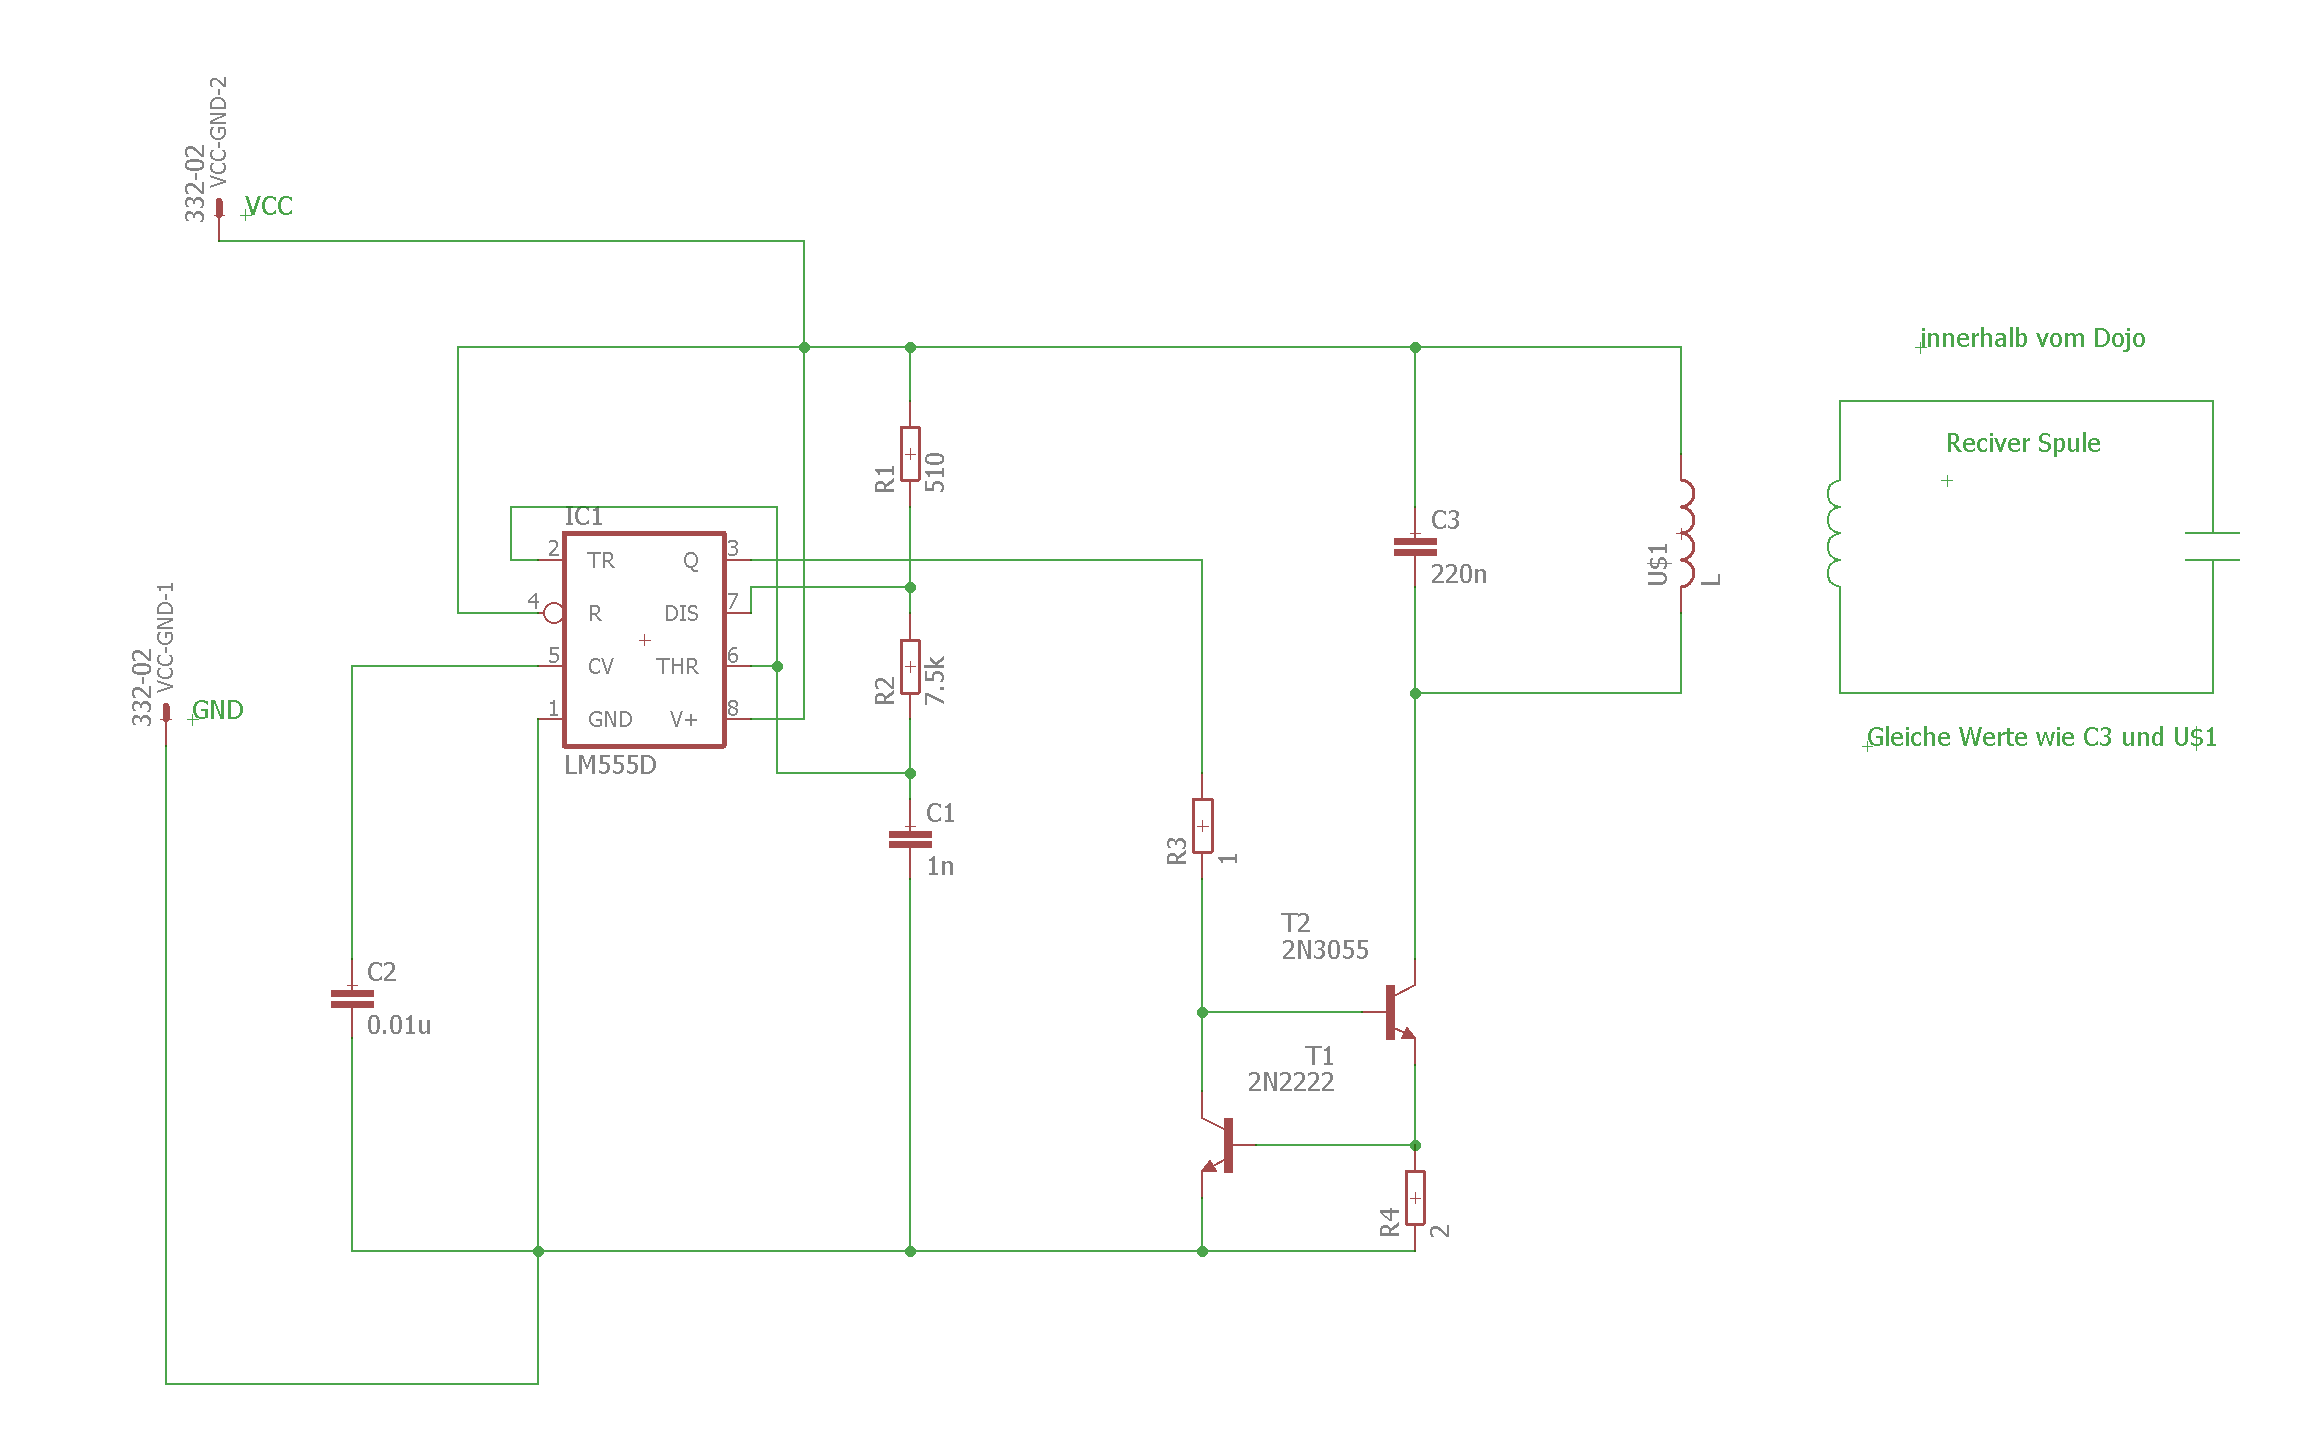
\includegraphics[width=\textwidth]{data/Tranceiver.png}
		\caption[Ne555]{Die verwendete Timerschaltung als Pulsquelle} %picture caption
		\label{fig:Tranceiver-Schaltung}
	\end{center}
\end{figure}
 
Das Pulssignal selber muss verschiedene Kriterien erfüllen. Zum einen sollte der Duty Cycle so nahe wie möglich an $50\%$ sein. Um dies zu erreichen muss $R2 >> R1$ gelten. Das andere Kriterium ist die Erreichung der Resonanzfrequenz des LC-Gliedes. Um das Pulssignal optimal einzustellen, können folgende Richtlinien betrachtet werden:
\begin{description}
	\item [$\cdot$ C] beeinflusst die Zeiten (Frequenz/High-Time/Low-Time)
	\item [$\cdot$ R$_{1}$] beeinflusst die High-Time, lässt jedoch die Low-Time unverändert.
	\item [$\cdot$ R$_{2}$ ] beeinflusst die High- und Low-Time und beeinflusst somit den Duty Cycle.
\end{description}

Die verwendeten Komponenten $C$, $R_{1}$ und $R_{2}$ wurden durch nachfolgende Formeln \ref{eq:Timerf} bis \ref{eq:TimerR2} berechnet. 

\begin{equation}\label{eq:Timerf}
f= \dfrac{1}{T}= \dfrac{1.44}{((R_{1} + 2 \cdot R_{2})\cdot C)}
\end{equation}
\begin{equation}\label{eq:TimerTL}
LowTime= 0.693 \cdot R \cdot C
\end{equation}
\begin{equation}\label{eq:TimerTH}
HighTime= 0.693 \cdot (R_{1} + R_{2}) \cdot C
\end{equation}
\begin{equation}\label{eq:TimerDC}
D = DutyCycle = \dfrac{R_{1} + R_{2}}{R_{1} + 2 \cdot R_{2}}
\end{equation}
\begin{equation}\label{eq:TimerR1}
R1 = 1.44 \cdot \left( \dfrac{2 \cdot D - 1}{f \cdot C} \right)
\end{equation}
\begin{equation}\label{eq:TimerR2}
R2 = 1.44 \cdot \left( \dfrac{1-D}{f \cdot C} \right)
\end{equation} 

Für die Berechnung der effektiven Werte, müssen die ersten Werte angenommen werden. Nach der Anpassung und unter Berücksichtigung der E-Reihe, ergaben sich die folgenden Bauteilwerte für die angepasste Transceiverschaltung:

\begin{itemize}
\item C = $1nF$
\item R1 = $200\Omega$
\item R2 = $9k\Omega$
\end{itemize}
 
Gemäss Berechnung \ref{eq:Timerf} beträgt die Frequenz $79.12kHz$. Nach der Berechnung der Frequenz, können nun die einzelnen Komponenten ausgewählt und implementiert werden. Dabei gilt es zu beachten, dass minimale Abweichungen bereits zu einer Änderung der Frequenz, Pulsdauer und Duty-Cycle des Pulssignales führen.

\subsubsection*{Receiver}
Er besteht primär aus einem LC-Glied und einem Gleichrichter. Das verwendete LC-Glied ist das gleiche wie bei der Transceiverschaltung. Der Grund dafür liegt im kleinen Energiefeld. Der Receiver könnte dann im Falle einer grösseren Spule nicht optimal ausgenutzt werden. Die Flachspule lässt sich mit einer Dimension von $\o 15mm$ Durchmesser und $2mm$ Höhe gut im Inneren des Dōjōs platzieren. Die Positionierung findet am Boden statt und ermöglicht dadurch die besten Übertragungswerte von Strom und Spannung. Der benötigte Kondensator für die Vervollständigung des LC-Gliedes kann direkt hinter der Spule angebracht werden. Die hochfrequente Wechselspannung muss für die Speisung der Batterie noch gleichgerichtet werden. Hierbei werden sowohl Kondensatoren als auch spezielle Gleichrichterdioden verwendet, welche einen Spannungsabfall von lediglich $0.1V$ aufweisen. Anschliessend wird die gesamte Ladeschaltung gespiesen, welche den gesamten Ladeprozess des Akkus übernimmt. Einen Einblick in diesen Ladeprozess gibt nachfolgendes Kapitel.
